\documentclass[11pt, a4paper, openright, DIV12, BCOR=1cm]{scrbook}

\usepackage{scrhack} %Hacks around some old packages --> less warnings :-)

% language
\usepackage[american]{babel}
\usepackage[utf8]{inputenc}

% bib
\bibliographystyle{plainurl}

\usepackage{amsmath}
\usepackage{amsfonts}
\usepackage{amsthm}
\usepackage{url}

% I need them :-)
\usepackage[plainpages=false]{hyperref}
\hypersetup {
   pdfauthor={Johannes Wei\ss},
   pdftitle={Diplomarbeit Johannes Wei\ss},
   pdfsubject={Diploma Thesis},
   pdfkeywords={KIT, crypto, diploma thesis, Diplomarbeit, Informatik, computer
   science}
}
\usepackage{listings}
\usepackage{color}
\usepackage{tikz}

% DRAFT WATERMARK
\usepackage{draftwatermark}
\SetWatermarkText{DRAFT}
\SetWatermarkScale{4.0}


%
% SPECIAL IMPORTS
%
\usepackage{xparse}
\usepackage{boxedminipage}


%
% GENERAL
%

% environments
\NewDocumentEnvironment{JWboxed}{mm}%
  {\begin{figure}[ht]%
   \small%
   \begin{boxedminipage}{\linewidth}%
  }%
  {\end{boxedminipage}%
   \caption{#1}%
   \label{#2}%
   \end{figure}%
  }

% functionality
\newenvironment{JWfunc}[3]%
{\begin{JWboxed}{#2}{#3}%
 \begin{center}\textbf{{Functionality #1}}\end{center}%
}%
{\end{JWboxed}}

\newenvironment{JWfuncSteps}[0]%
{\begin{itemize}}{\end{itemize}}

\newcommand{\JWfuncSym}[2]{$\mathcal{F}^\mathrm{#1}_\mathrm{#2}$}

%protocol
\newenvironment{JWprotocol}[3]%
{\begin{JWboxed}{#2}{#3}%
 \begin{center}\textbf{{Protocol #1}}\end{center}%
}%
{\end{JWboxed}}

\newenvironment{JWprotoSteps}[0]%
{\begin{enumerate}}{\end{enumerate}}

\newcommand{\JWprotoPhase}[1]{\paragraph{#1}}

\newcommand{\JWprotoSym}[2]{$\Pi^\mathrm{#1}_\mathrm{#2}$}

%misc
\newcommand{\JWtodo}[1]{\fbox{TODO: #1}}
\newcommand{\JWmsgTwo}[2]{(\texttt{#1}, \texttt{#2})}

%chapters
\newcommand{\JWlone}[1]{\chapter{#1}}
\newcommand{\JWltwo}[1]{\section{#1}}
\newcommand{\JWlthree}[1]{\subsection{#1}}
\newcommand{\JWlfour}[1]{\subsubsection{#1}}
\newcommand{\JWlfive}[1]{\paragraph{#1}}
\newcommand{\JWlsix}[1]{\subparagraph{#1}}


%
% SPECIALIZED SHORTCUTS
%
\newcommand{\JWprotoSymOPE}[0]{\JWprotoSym{}{OPE}}
\newcommand{\JWfuncSymOPE}[0]{\JWfuncSym{(q, k)}{OPE}}
\newcommand{\JWfieldGeneral}[0]{\mathbb{F}_q^k}
\newcommand{\JWpOne}[0]{Goliath}
\newcommand{\JWpTwo}[0]{David}


\title{Efficient Secure Function Evaluation using Garbled Arithmetic Circuits
and Untrusted Tamper--Proof Hardware}

\author{Johannes Weiß}

\begin{document}

\selectlanguage{american}

\pagenumbering{Roman}

\maketitle

\vspace*{\fill}

\noindent{}{\Large Eigenst\"andigkeitserkl\"arung}

\bigskip{}

\noindent{}Hiermit versichere ich, dass ich die Arbeit selbst\"andig verfasst
habe und keine anderen als die angegebenen Quellen und Hilfsmittel benutzt habe,
die w\"ortlich oder inhaltlich \"ubernommenen Stellen als solche kenntlich
gemacht habe und die Satzung des Karlsruher Instituts f\"ur Technologie zur
Sicherung guter wissenschaftlicher Praxis in der g\"ultigen Fassung beachtet
habe.

\bigskip{}

Karlsruhe, den 17. Dezember 2012 \JWtodo{Datum fixen}

\bigskip{}

\bigskip{}
Johannes Wei\ss

\vspace*{\fill}

\cleardoublepage

\vspace*{\fill}
\begin{center}
{\Large \JWtitle{}} \\
Johannes Wei\ss{} $<$diplomarbeit@johannesweiss.eu$>$
\end{center}
\vspace*{\fill}

\newpage

\null
\vfill
\hfill Typeset using \LaTeX{} on \today{}, \currenttime{}.
\input{res/git-state.tex}


\frontmatter
\tableofcontents

\mainmatter

\cleardoublepage

\JWlone{Introduction}
\label{sec:introduction}

An \JWdef{Secure Multi--Party Computation}{MPC} or \JWdef{Secure Function
Evaluation}{SFE} is the joint calculation of an arbitrary function $f$ with
private inputs from a set of mutually distrusting parties. If the size of the
set of parties for an MPC is $2$, the computation is also called a two--party
computation. The area of research of secure multi--party computations was
founded by \emph{Yao's Millionaires' Problem} \cite{yao82}. The famous
Millionaires' Problem discusses two millionaires, who are interested in knowing
which of them is richer without revealing the actual values of their wealth. The
problem is evaluating the function $f(a, b) = a \geq b$, where the first
millionaire inputs the value of his wealth as $a$ and the second inputs $b$. The
result of the evaluation is either \textit{false} if the second millionaire is
richer or \textit{true} meaning the opposite. From the result and the own input,
neither party is able to calculate the wealth of the other millionaire. Another
example for real--world multi--party computations are democratic elections. The
eligible voters input their private vote and the result of the calculations is
the percentage breakdown.

\JWdefn{Oblivious Polynomial Evaluation}{OPE} \cite{naor99,naor06} is a special
case of SFE. In contrast to arbitrary functions that are known by the involved
parties, OPE only allows the first party to privately submit a polynomial $p$
and another party to evaluate the polynomial at one node $x$. The second party
obtains the result $p(x)$ without revealing $x$ to the first party or revealing
the polynomial $p$ to the second party. We find a secure and efficient OPE
protocol a useful and interesting primitive. Many other cryptographic problems
can be based on OPE, for example the share generation for \emph{Shamir's Secret
Sharing} \cite{shamir79}.

\JWdefn{Oblivious Affine Function Evaluation}{OAFE} \cite{davidgoliath} is a
primitive that allows---similar to OPE---to obliviously evaluate affine
functions. The David \& Goliath protocol \cite{davidgoliath} presents a secure
and efficient OAFE implementation based on only one stateful tamper--proof
hardware token. Based on OAFE, this thesis works out the astonishing result of
OPE in linear time which is asymtotically as fast as usual polynomial
evaluation. Alongside the theoretical methodology, this thesis features an
efficient, secure, and working implementation of the proposed protocol. The
presented approaches are also suitable for general SFE (including \emph{Square
\& Multiply} \cite{knuth81}), however the security is only proved for OPE. The
security of the protocol against passive and active adversaries is
in\-for\-ma\-tion--the\-o\-ret\-ically proved in the \JWdefn{Universal
Composability}{UC} framework \cite{canetti05}. \JWtodo{Hier alle Beiträge meiner
Arbeit reischreiben}


%
% RELATED WORK
%
\JWltwo{Related Work}
\label{sec:related-work}

The notion of \emph{universal composability} in the UC framework by Canetti
\cite{canetti05} places strict demands on the security of cryptographic
protocols. Proofs in the UC framework have to show that any environment is
unable to distinguish between an ideal functionality and the actually
implemented protocol, even when malicious adversaries misuse the protocol in
some unpredictable way. The benefit of the strict requirements of this notion is
that UC--secure protocols can be composed and ran concurrently while still
staying safe without the necessity of additional security proofs. This thesis
states universal composability as the notion of security.

Yao defined the problem of multi--party computations and his \JWdefn{Garbled
Circuit}{GC} approach \cite{yao86} describes encrypted evaluation of (boolean)
circuits. But despite the versatility of Yao's garbled circuits, the approach is
not suitable for arithmetic functions on large fields. Because the GC approach
requires embedded truth tables in every gate, an adoption to larger finite
fields would have the consequence of a quadratic blowup of every truth table in
every gate (cf.\ \cite{naor99privacy}). This thesis solves these problem
efficiently for arbitrary polynomials.

Besides the GC approach, this thesis is also related to \emph{Efficient
Multi-Party Computation Over Rings} by Cramer et al.\cite{cramer03}. The
difference is that Cramer's approach is based on the simulation of formulas by
bounded--width programs by Cleve \cite{cleve91} which does not support
\emph{Square \& Multiply} \cite{knuth81} and the complexity is slightly
polynomial in the number of arithmetic operations performed. The writings of
Naor et al.\cite{naor99,naor06} also describe OPE but are in polynomial
complexity and based on \JWdefn{Oblivious Transfer}{OT} \cite{rabin81}.

\emph{How to Garble Arithmetic Circuits} by Applebaum et al.\cite{gac2012}
describes the garbled evaluation of arithmetic circuits.  Many ideas used in
this thesis are inspired by Applebaum et al. The difference between the
Applebaum's paper and this thesis, is that the former relies on computational
assumptions. In contrast, this thesis does not rely on computational assumptions
and proves the methodology to be information--theoretically secure. This thesis
switches some of Applebaum's ideas to \JWdefn{Oblivious Affine Function
Evaluation}{OAFE} \cite{davidgoliath}.

%
% ACKNOWLEDGMENTS
%
\JWltwo{Acknowledgments}

I wish to thank my advisor Daniel Kraschewski who supported me throughout the
research and writing of this thesis. He donated a large amount of his limited
time for discussions and explorations crucial for my thesis and allowed this
thesis to be my own work but steered me in the right direction when needed.  I
am also thankful for his patience introducing me to this exciting topic.


%
% Outline
%
\JWltwo{Outline}

This thesis starts by introducing the reader to the general methodology, which
is discussed in depth thereafter (Chapter \ref{sec:methods}). Next, the security
of the methodology is analyzed and proved in the UC framework (Chapters
\ref{sec:protocol} and \ref{sec:security}). Since this thesis also implements
the proposed protocol, the implementation is covered (Chapter
\ref{sec:implementation}). An evaluation of both, the methodology and the
implementation (Chapter \ref{sec:evaluation}) rounds out this thesis.  And since
a large amount of the time taken for this thesis was affected by researching, a
quick tour of the alternative approaches is given to the reader (Chapter
\ref{sec:discontinued}).

% vim: set spell spelllang=en_us fileencoding=utf8 formatoptions=tcroql : %


\JWlone{Methods}
\label{sec:methods}

This chapter describes how arbitrary arithmetic functions can be expressed in
terms of affine expressions. This is the most important part of this thesis
because it is the key part of evaluating arbitrary arithmetic expressions
using OAFEs \cite{davidgoliath}.


%
% DEFINITIONS
%
\JWltwo{Definitions}
\label{sec:rae-definitions}

This chapter defines important entities that are used to define the more complex
entities in the following chapters.

% Field K
\JWlthree*{Field $K$}

\label{def:field} Throughout this thesis, $K$ represents an arbitrary finite
field, such as $\mathbb{F}_{2^{256}}$.


% Variables
\JWlthree*{Variables}

\label{def:variable} Variables are textual placeholders for real values.
Formally represented by

\begin{align*}
  \mathcal{V} = & \{ x \mid x~\text{a variable that can be set to an element
  $e$}, e \in K \}
\end{align*}


%
% DUAL RANDOMIZED AFFINE VALUES
%
\JWltwo{Dual Randomized Affine Values}
\label{sec:drav}

\JWdef{Dual Randomized Affine Value}{DRAV}{s} are encrypted, signed values
representing a scalar value of the field $K$. Each DRAV is encrypted by a pair
of \emph{dual keys}. The first dual key, the \emph{static key}, remains the same
in the whole DRAC (see chapter \ref{def:DRAC}) generation procedure and is
usually written as $(\alpha_l, \alpha_r)$. The second dual key, the
\emph{dynamic key} is a short--lived key, usually represented as $(\beta,
\beta')$. Two DRAVs only share the same dynamic key by hazard but always share
the same static key. Encoding a regular value $v \in K$ as a DRAV
$\widetilde{v} \in \mathcal{V}_K$ is very simple:

\begin{align*}
  \widetilde{v} = E(v) = (\widetilde{v_l}, \widetilde{v_r}) =
    (\alpha_l \cdot v + \beta, \alpha_r \cdot v + \beta')
\end{align*}

So if the keys are uniformly at random, the two components of the tuple
$\widetilde{v}$ are uniformly at random, too. Decoding is:

\begin{align*}
  v = D(\widetilde{v}) =
  \left\{
    \begin{array}{l l}
      \frac{\widetilde{v_l} - \beta}{\alpha_l} & \quad
      \text{if}~\frac{\widetilde{v_l} - \beta}{\alpha_l} =
      \frac{\widetilde{v_r} - \beta'}{\alpha_r}\\
      \bot & \quad \text{otherwise ($\widetilde{v}$ is non--well--formed)}\\
    \end{array}\right.
\end{align*}

\begin{JWtodoBox}
  \begin{itemize}
    \item Was ist well--formedness, non--well--formedness?
    \item Final Value evaluation, also Addieren der Komponenten
    \item Arithmetic auf DRAVs (kann man aus dem alten CBRAE Kapitel klauen)
  \end{itemize}
\end{JWtodoBox}


% DIRECT DRAV ARITHMETIC
\JWlthree{Direct DRAV Arithmetic}

Direct DRAV arithmetic only supports addition ($+$) of two DRAVs. Indirect DRAV
arithmetic has to be used for other operations. The advantage of direct DRAV
arithmetic is that it can be performed without the knowledge of a DRAV's
encryption keys.


\paragraph{Addition of Well--Formed DRAVs:} Two DRAVs $\widetilde{x} =
(\widetilde{x_l}, \widetilde{x_r})$ and $\widetilde{y} = (\widetilde{y_l},
\widetilde{y_r})$ can be added componentwise to $\widetilde{z} =
\left(\widetilde{x_1} + \widetilde{y_1}, \widetilde{x_2} +
\widetilde{y_2}\right)$. The encryption keys for $\widetilde{z}$ will be
$(\alpha_l, \alpha_r)$ and $(\beta_1 + \beta_3, \beta_2 + \beta4)$ assuming
$\widetilde{x}$ was encrypted with $(\alpha_l, \alpha_r)$ and $(\beta_1,
\beta_2)$ and $y$ was encrypted with $(\alpha_l, \alpha_r)$ and $(\beta_3,
\beta_4)$.

\subparagraph{Proof:} From ($\widetilde{x} = \left(\alpha_l \cdot x + \beta_1,
\alpha_r \cdot x + \beta_2\right)$, $\widetilde{y} = \left(\alpha_l \cdot x +
\beta_3, \alpha_r \cdot x + \beta_4\right)$) it's obvious that: $\widetilde{z} =
\left(\alpha_l \cdot (x+y) + (\beta_1 + \beta_3), \alpha_r \cdot (x+y) +
(\beta_2 + \beta_4)\right)$ and $\widetilde{z}$ is well--formed.

\paragraph{Addition of Non--Well--Formed DRAVs:} It's of particular interest the
following property holds: $\forall \widetilde{x}: \widetilde{x} + \bot = \bot
+ \widetilde{x} = \bot$. Let $\widetilde{\chi}$ be a non--well--formed DRAV,
so: $\widetilde{\chi} = (\alpha_l \cdot \chi + \beta_3 + \Delta_l, \alpha_r
\cdot \chi + \beta_4 + \Delta_r)$. The component--wise addition
$\widetilde{\nu}$ of $\widetilde{\chi}$ to any well--formed $\widetilde{x} =
(\alpha_l \cdot x + \beta_1, \alpha_r \cdot x + \beta_2)$ is $\widetilde{\nu} =
(\alpha_l \cdot (x+\chi) + (\beta_1+\beta_3) + \Delta_l, \alpha_r \cdot (x+\chi)
+ (\beta_2+\beta_4) + \Delta_r)$. Using the universal decoding function $D$, the
value of $\chi$ is $\chi = D(\widetilde{\chi}) = (x + \chi +
\frac{\Delta_l}{\alpha_l}, x + \chi + \frac{\Delta_r}{\alpha_r})$. So: $\forall
(\Delta_r, \Delta_l) \in K \setminus \{(0, 0)\} \wedge \frac{\Delta_l}{\alpha_l}
\neq \frac{\Delta_r}{\alpha_r}: D(\widetilde{\chi}) = \bot$. Since the
encryption keys are not known to an attacker, $\frac{\Delta_l}{\alpha_l} \neq 0
\wedge \frac{\Delta_r}{\alpha_r}$ hold except for a negligible probability if
$\Delta_r \neq 0 \vee \Delta_r \neq 0$ and that's the property for being forged
(non--well--formed) which was the assumption. Trivially $\bot + \bot = \bot$ by
a similar argument.


% INDIRECT DRAV ARITHMETIC
\JWlthree{Indirect DRAV Arithmetic}
\label{sec:drac-arithmetic}

Indirect DRAV arithmetic assumes the universal encoding and decoding functions
$E(v)$ and $D(\widetilde{v})$ and therefore the knowledge of the encryption
keys. Another possibility is to map indirect DRAV arithmetic to OAFE calls that
are set up by a party that knows the encryption keys.


% FINAL DRAV DECODING
\JWlthree{Final DRAV Decoding}
\label{sec:drav-final-decoding}

Finally decoding a DRAV can be trivially done using the universal decoding
function $D(\widetilde{v})$. But $D$ is only available to a party that is in
possession of the encryption keys.

Additionally a DRAV can also be finally decoded only one additional OAFE call.
The following procedure will decode a DRAV to a final scalar value although
$D$ is a partial function. To enable a second party---that is not in possession
of the encryption keys---to decode a DRAV $\widetilde{v} = (\widetilde{v_1},
\widetilde{v_2})$, the first party---in possession of the keys---needs to set up
a special OAFE, called the \emph{final OAFE} below.

The second party's input to the final OAFE is $\widehat{v} = \widetilde{v_1} +
\widetilde{v_2}$, the addition of both components of the DRAV to decode.  The
final OAFE was set up by the first party as follows: Assuming $\widetilde{v}$ is
encrypted by $(\alpha_l, \alpha_r)$ and $(\beta_1, \beta_2)$ the first party
knows $\widehat{v}$ has to be encrypted using $(\alpha_l + \alpha_r)$ and
$(\beta_1 + \beta_2)$.  Given this knowledge the final OAFE setup is
$\frac{1}{\alpha_l + \alpha_r} \cdot \widehat{v} - \frac{\beta_1 +
\beta_2}{\alpha_l + \alpha_r}$.

Again, it's important that an attacker is getting caught when trying to forge a
DRAV ($D(\widetilde{v}) = \bot$ if $\widetilde{v}$ has been forged, $\bot$ is
mapped to uniform randomness in this process since an OAFE has no
$\bot$--value). If the attacker cheated somewhere in the process and forged one
of the DRAV tuples $\widetilde{x} = (\widetilde{x_1}, \widetilde{x_2})$ to
$\widetilde{x'} = (\widetilde{x_1} + \Delta_1, \widetilde{x_2} + \Delta_2)$, the
DRAV $\widetilde{x'}$ becomes---except for a negligible
probability---non--well--formed (see section \ref{sec:drav}). The result is that
the decoded result will become uniform randomness (assuming $\widetilde{x}$ is
forged to $\widetilde{x'_1} = \widetilde{x_1} + \Delta_1$ and $\widetilde{x'_2}
= \widetilde{x_2} + \Delta_2$):

\begin{align*}
  \widehat{x'} = & \widetilde{x'_1} + \widetilde{x'_2} = \widetilde{x_1} +
  \Delta_1 + \widetilde{x_2} + \Delta_2 \\
  %
  \Rightarrow x' = & \frac{1}{\alpha_l + \alpha_v} \cdot \widehat{x'} -
  \frac{\beta_{x_1} +
  \beta_{x_2}}{\alpha_l + \alpha_v} \\
  %
  \Leftrightarrow x' = & \frac{\widetilde{x_1} + \Delta_1 +
  \widetilde{x_2} + \Delta_2}{\alpha_l + \alpha_v} -
  \frac{\beta_{x_1} +\beta_{x_2}}{\alpha_l + \alpha_v}\\
  %
  \Leftrightarrow x' = & \frac{(\alpha_l x + \beta_{x_1}) + \Delta_1 +
  (\alpha_v x + \beta_{x_2}) + \Delta_2}{\alpha_v + \alpha_l} -
  \frac{\beta_{x_1} +\beta_{x_2}}{\alpha_l + \alpha_v} \\
  %
  \Leftrightarrow x' = & \frac{(\alpha_l+\alpha_v)x + (\beta_{x_1}+\beta_{x_2} +
  \Delta_1+\Delta_2)}{\alpha_l+\alpha_v} -
  \frac{\beta_{x_1} +\beta_{x_2}}{\alpha_l + \alpha_v} \\
  %
  \Leftrightarrow x' = & x + \frac{\beta_{x_1}+\beta_{x_2}}{\alpha_l+\alpha_v}
  + \frac{\Delta_1 + \Delta_2}{\alpha_l + \alpha_v} -
  \frac{\beta_{x_1}+\beta_{x_2}}{\alpha_l + \alpha_v} \\
  %
  \Leftrightarrow x' = & x + \frac{\Delta_1 + \Delta_2}{\alpha_l + \alpha_v}\\
\end{align*}

Because an attacker is not in possession of the static encryption keys
$\alpha_l$ and $\alpha_r$, it cannot control the value of $\frac{\Delta_1 +
\Delta_2}{\alpha_l + \alpha_r}$. Since $\alpha_l$ and $\alpha_r$ are chosen
uniform at random, the result $x'$ becomes uniform at random, too.


%
% DUAL RANDOMIZED AFFINE ENCODING
%
\JWltwo{Dual Randomized Affine Encoding}
\label{sec:drae}

\JWdef{Dual Randomized Affine Encoding}{DRAE}{s} are affine representations of
parts of arithmetic circuits that fulfill several properties:

\begin{enumerate}

  \item \label{prop:drae-encrypted} DRAEs are encrypted: Without the encryption
    keys, they don't reveal any information.

  \item \label{prop:drae-signed} DRAEs are signed: If someone tries to forge a
    DRAE, it will become non--well--formed and operations with that DRAE result
    in non--well--formed DRAEs.

  \item \label{prop:drae-oafe} DRAEs can be securely evaluated using OAFEs.

  \item \label{prop:drae-not-enough} DRAEs can not express arbitrary arithmetic
    circuits alone.

\end{enumerate}

\noindent{}A DRAE can be eventually evaluated to a final value, that is a DRAV
(see chapter \ref{def:DRAV}).


%
% DUAL RANDOMIZED AFFINE CIRCUITS
%
\JWltwo{Dual Randomized Affine Circuits}
\label{sec:drac}

\JWdef{Dual Randomized Affine Circuit}{DRAC}{s} are representations of entire
arbitrary arithmetic circuits. DRACs are sequences of DRAEs, each assigned to a
variable.

% EVALUATION
\JWlthree{Evaluation}
\label{sec:DRAC-eval}

A DRAC can be evaluated by evaluating one DRAE after the other and assigning the
resulting DRAV to the variable the DRAE is assigned to. The DRAE sequence is
ordered, so a DRAE can be evaluated by only inputting the regular inputs
and the variables set by evaluating prior DRAEs. The last DRAV can then be
decoded as explained in chapter \ref{sec:drav-final-decoding}.


\JWltwo{DRAEs weiter...}

are very similar to AREs
(section \ref{sec:are}) but use CBRVs (section \ref{sec:cbrv}) instead of plain
values and RVs (section \ref{sec:rv}). \ref{def:LW} \ref{def:AW}

\begin{align}
  \mathcal{F}_{AR} = & \{ s \cdot x + i \mid s, i \in K, x \in \mathcal{V} \}
  \cup \{ v \mid v \in K \} \\
%
  \mathcal{B}_{AR} = & \{ (\alpha_l \cdot f + \beta, \alpha_r \cdot f + \beta' )
  \mid \alpha_l, \alpha_r \in K \setminus \{0\}; \beta, \beta' \in K; f \in
  \mathcal{F}_{AR} \} \\
%
  \label{rel:drae}
  \mathcal{E}_{AR} = & \{ (M, A) \mid
    M \subseteq \mathcal{B}_{AR} \times \mathcal{B}_{AR},
    A \subseteq, \mathcal{B}_{AR};
    A, M~\text{finite multi--sets} \}
%
\end{align}

\noindent Intuitively, $\mathcal{V}$ are ordinary inputs and CBRVs,
$\mathcal{F}_{AR}$ represent linear, encrypted particles that encode parts of
the final function. To prevent illegal information gaining by a corrupted second
party, $\mathcal{B}_{AR}$ represents checked and encoded intermediate values
(see section \ref{sec:cbrv}) that can safely be passed to untrusted parties.
$\mathcal{E}_{AR}$ is the final encoding, powerful enough to encode arbitrary
arithmetic functions. $\mathcal{E}_{AR}$s are full--blown DRAEs as presented in
this thesis. The decoding part remains as in section
\ref{sec:affinization_decoding}. The result will be a tuple that can then be
decoded in one last step as in section \ref{sec:eval-final-value}.


\JWlthree{Encoding Arithmetic Operations as DRAEs}
\label{sec:encode-drae}

\JWlfour{Addition}

Having two DRAEs, they can be added by simply concatenating the multiplicative
($M$ in relation \ref{rel:drae}) and additive ($A$) parts.


\JWlfour{Addition -- Alternative Form}

The alternative addition form is
$\widetilde{z} =
\left( E\left(D(\widetilde{x_1}) + D(\widetilde{y_1})\right),
       E\left(D(\widetilde{x_2}) + D(\widetilde{y_2})\right)
\right)$.
Since $E(x)$ and $D(x)$ are both linear functions,
$E\left(D(\ldots) +D(\ldots)\right)$
are linear expressions, too that can be evaluated using two OAFE calls.


\JWlfour{Multiplication}

As for ordinary AREs, the multiplication is not as powerful as the addition,
direct multiplication of two DRAEs is not possible. DRAE multiplication is
done using CBRVs sent to the second party. Then, these CBRVs get multiplied as
described here:

\begin{align*}
  e & \in \mathcal{E}_{AR}; \widetilde{x}, \widetilde{y} \in \mathcal{B}_{RV};
  r_1, r_2, r_3, r_4, r_5, r_6, r_7, r_8 \in K;
  \alpha_l, \alpha_r \in K \setminus \{0\} \\
  %
  e & = \widetilde{x} \otimes \widetilde{y} \\
  %
  e & = \Bigg(\Big\{\big( \alpha_l \cdot D(\widetilde{x_1}) - r_1,
                          \alpha_r \cdot D(\widetilde{x_2}) -r_5 \big) \\
    &\qquad ,     \big(   1        \cdot D(\widetilde{y_1}) - r_2,
                          1        \cdot D(\widetilde{y_2}) - r_6 \big) \Big\}\\
    &\qquad   \Big\{\big( \alpha_lr_2 \cdot D(\widetilde{x_2}) + r_3,
                          \alpha_rr_2 \cdot D(\widetilde{x_1}) + r_7 \big) \\
    &\qquad ,       \big ( r_1        \cdot D(\widetilde{y_2}) + r_4,
                           r_5        \cdot D(\widetilde{y_1}) + r_8 \big)
              \Big\}\Bigg) \\
\end{align*}

The decryption keys of $e$ are $\alpha_l$, $\alpha_r$ (static keys) and
$\beta = r_1r_2 + r_3 + r_4$, $\beta' = r_5r_6 + r_7 + r_8$ (dynamic keys).

\JWltwo{Checked Bi--Randomized Variables}
\label{sec:cbrv}

The RV technique (see section \ref{sec:rv}) prevents the
second party from directly gaining intermediate information. But, for a
corrupted second party, there is still the possibility of gaining supplemental
information: The second party could forge an RV value before applying it to one
of the following AREs. This will not directly reveal additional information
because the second party does not know the encryption keys used for the RV. So,
the second party is unaware of the decoded value of the RV. But except for a
negligible probability $\left(\frac{1}{Char(K)}\right)$, the decoded value is
non--zero.  The knowledge of a random but non--zero value can then be used to
test a secret input of the first party against zero. \JWtodo{Beispiel hierfür,
siehe z.B. Google Doc.}

To address this issue, a similar but secure technique is proposed in here: The
\emph{Checked Bi--Randomized Variables} (CBRVs). Every input made to an OAFE by
the second party is encoded as a CBRV. The CBRVs $\hat{v}$ corresponding to a
value $v$ are: ($\alpha_l, \alpha_r \in K \setminus \{0\}; \beta, \beta' \in K$)

\begin{align*}
  \widetilde{v} = (\widetilde{v_1}, \widetilde{v_2}) =
  (\alpha_l \cdot v + \beta, \alpha_r \cdot v + \beta')
\end{align*}

\noindent{} $\alpha_l$ and $\alpha_r$ are the \emph{static keys}, $\beta$ and
$\beta'$ the \emph{dynamic keys} of the CBRV. The static keys are (non--zero)
numbers uniformly at random but constant for the entire procedure. $\beta$ and
$\beta'$ are fresh, independent and uniformly distributed random numbers for
every CBRV component generated while processing a circuit. Only the first party
knows these secret keys. The initial CBRVs used to feed the second party's
regular inputs party are generated using an OAFE that evaluates for every input
$x$:

\begin{align*}
  \widetilde{x} = (\alpha_l \cdot x + \beta_1, \alpha_r \cdot x + \beta_2)
\end{align*}

The first party is---because it generates and knows all the keys---in possession
of the encoding and decoding functions

\begin{align*}
  E(x) &= \left(\alpha_l \cdot x + \beta_1, \alpha_r \cdot x + \beta_2\right) \\
  D(\widetilde{x}) &= \left(\frac{\widetilde{x_1} - \beta_1}{\alpha_l},
                       \frac{\widetilde{x_2} - \beta_2}{\alpha_r}\right)
\end{align*}

A CBRF $\widetilde{x}$ is well--formed iff the tuple $D(\widetilde{x})$ consists
of two equal values.




%
% PREPARING DRAE EVALUATION USING OAFEs
%
\JWltwo{Preparing DRAE Evaluation Using OAFEs}
\label{sec:prep-eval}

After transforming an arithmetic expressing to DRAEs (section \ref{sec:drae})
assigned to CBRVs (section \ref{sec:cbrv}) the OAFEs (\cite{davidgoliath}) need
to be set up. First of all, two separate OAFEs have to be set up for each CBRV
that can be evaluated later on as soon the value is known. The OAFEs are
configured with the linear expressions inside the DRAEs. Each DRAE is then
transformed to two \emph{Encoding Descriptors} (EDs) that have the same
structure as the DRAEs but contain OAFE references instead of linear
expressions. Therefore, each DRAE assigned to a CBRV gets transformed to two
EDs, because of the tuple form of the CBRVs and DRAEs.


%
% OBLIVIOUS POLYNOMIAL EVALUATION
%
\JWltwo{Oblivious Polynomial Evaluation}
\label{sec:ope}

This section describes the whole process of obliviously evaluating a univariate
polynomial $f(x) = \sum_{i=1}^k a_ix^i$. The first party (\JWpOne{}) fixes the
polynomial and configures the OAFEs, the second party (\JWpTwo{}) chooses input
$x$. Eventually, \JWpTwo{} will learn $f(x)$ but not the polynomial's
coefficients $a_i$. \JWpOne{} will not learn anything at all.

The first step is to transform $f$ to OAFEs and EDs (section
\ref{sec:prep-eval}). The OAFEs are then sent to the second party (\JWpTwo{})
using the David \& Goliath protocol \cite{davidgoliath}, the EDs are sent to the
second party using an encrypted channel aswell.

After having received the OAFEs and EDs, the first party (\JWpOne{}) is not
needed anymore and the second party (\JWpTwo{}) can evaluate the polynomial by
itself. To run the evaluation, the second party just evaluated the EDs one by
one. After each evaluation, it queries the respective OAFE (should be the next)
with the value if did just calculate. After having calculated the last to ED
values, it queries a special OAFE (see section \ref{sec:eval-final-value}) using
the addition of the values of the last two EDs. The evaluation of the special
OAFE is the result of the whole computation.

% vim: set spell spelllang=en_us fileencoding=utf8 :


%
% PROTOCOL DESCRIPTION
%
\JWlone{Protocol Description}
\label{sec:protocol}

\begin{JWfunc}%
  {\JWfuncSymOPE}%
  {The ideal $\JWfieldGeneral{}$-OPE functionality \JWfuncSymOPE{}}%
  {fig:func-ope}

  Parametrized by a finite field size $q$ and maximal polynomial degree $k$.

  \begin{JWfuncSteps}

  \item Upon receiving input $a \in \mathbb{F}_q^k$ from \JWpOne{}, verify that
    there is no stored input from \JWpOne{}, yet; else ignore that input. Next
    record $a$ and send \JWmsgTwo{processing}{\JWpOne{}} to the adversary.

  \item Upon receiving input $x \in \mathbb{F}_q$ from \JWpTwo{}, verify that
    there is no stored input from \JWpTwo{}, yet; else ignore that input. Next
    record $x$ and send \JWmsgTwo{processing}{\JWpTwo{}} to the adversary.

  \item Upon receiving a message \JWmsgTwo{delivery}{\JWpTwo{}} from the
    adversary, verify that \JWpTwo{} and \JWpOne{} have both already provided
    some input; else ignore that message. Next, compute $y \leftarrow
    \sum_{i=1}^k a_ix^i$ and send $y$ to \JWpTwo{}.

  \end{JWfuncSteps}
\end{JWfunc}

\begin{figure}[ht]

  \label{fig:graph-ope}
  \centering

  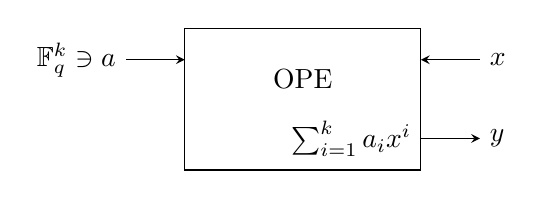
\begin{tikzpicture}[>=stealth]

    \node (OPE) at (8.5,0) {OPE};
    \draw (OPE) +(-1.5,-1.15) rectangle +(1.5,0.65);

    \draw [<-] (OPE) ++(-1.5,0.25) node [anchor=west] {} -- +(-0.75,0) node
    [anchor=east] {$\JWfieldGeneral \ni a$};

    \draw [<-] (OPE) ++(1.5,0.25) node [anchor=east] {} -- +(0.75,0) node
    [anchor=west] {$x$};

    \draw [->] (OPE) ++(1.5,-0.75) node [anchor=east] {$\sum_{i=1}^k a_ix^i$}
    -- +(0.75,0)
    node [anchor=west] {$y$};

  \end{tikzpicture}

  \caption{Graphical Representation of \JWfuncSymOPE}

\end{figure}

\begin{JWprotocol}%
  {\JWprotoSymOPE}%
  {Protocol: Oblivious Polynomial Evaluation}%
  {fig:proto-ope}

  \JWprotoPhase{Setup:}

  \begin{JWprotoSteps}

  \item \JWpOne{} generates the DRAC and sets up the OAFE functionality (see
    section \ref{sec:OPE}).

  \item \JWpOne{} sends DRAC to \JWpTwo{}.

  \end{JWprotoSteps}


  \JWprotoPhase{Evaluation:}

  \begin{JWprotoSteps}

  \item Upon receiving the DRAC, \JWpTwo{} verifies the received input really it
    a DRAC, else ignore that input. Additionally it verifies that the DRAC
    encodes a function whose degree is less or equal than the parametrized
    degree (see chapter \ref{sec:max-poly-degree}), else ignore the input.

  \item After a successful verification, \JWpTwo{} evaluates the DRAC, one DRAE
    after the other. Each DRAE evaluation leads to a DRAV that \JWpTwo{} stores
    as a variable that is used for further computations. Because the OAFE
    functionality is set up by \JWpOne{}, during the evaluation it is possible
    that the OAFE functionality turns out to behave unexpectedly: It could
    decline needed evaluations and it could return vectors of unexpected shapes.
    In both cases always assume it would have returned all zero vectors of the
    expected shape.

  \item After the Evaluation, \JWpTwo{} adds both components of the last DRAV
    and queries a special final OAFE with that value. The then received new
    value is the result of the computation $y = \sum_{i=1}^k a_ix^i$.

  \end{JWprotoSteps}

\end{JWprotocol}

% vim: set spell spelllang=en_us fileencoding=utf8 :


\JWlone{Correctness and Security of the Protocol}
\label{sec:security}

This chapter proofs the UC \cite{canetti05} security of the protocol described
in chapter \ref{sec:protocol}. Informally, the goal is to proof that for every
adversary $\mathcal{A}$ there has to exist a simulator $\mathcal{S}$ such that
for all environments $\mathcal{Z}$ the ideal functionality is indistinguishable
from the real protocol. Formally this can be represented as

\begin{align*}
%
\forall \mathcal{A}\ \exists \mathcal{S}\ \forall \mathcal{Z} :
\text{ideal}\ \widetilde{=}\ \text{real}
%
\end{align*}

%
% SIMULATORS
%
\JWltwo{Simulators}
\label{sec:simulators}


% SIMULATOR S_DAVID(A)
\JWlthree{Simulator $\mathcal{S}_{\text{\JWpTwo{}}}(\mathcal{A})$}
\label{sec:simulator-david}

\begin{itemize}

  \item Setup emulated honest \JWpTwo{}

  \item Feed emulated honest \JWpTwo{} with the same inputs the corrupted
    \JWpTwo{} receives

  \item Compare the outputs of the emulated, honest \JWpTwo{} with the corrupted
    one

  \item Should the corrupted \JWpTwo{} behave different than the emulated
    \JWpTwo{}, return uniform randomness as the final output to the environment

  \item Should the corrupted \JWpTwo{} behave honestly, pass it's input to the
    ideal functionality and output the return value to the environment

\end{itemize}


% SIMULATOR S_Goliath(A)
\JWlthree{Simulator $\mathcal{S}_{\text{Goliath}}(\mathcal{A})$}
\label{sec:simulator-goliath}

\begin{itemize}

  \item Setup an emulated, honest \JWpOne{}

  \item Feed the emulated \JWpOne{} with the same inputs the corrupted \JWpOne{}
    receives

  \item

\end{itemize}


%
% PROOF
%
\JWltwo{Security Proof}
\label{sec:proof}

The proof is a case distinction.


% CORRECTNESS --- BOTH PARTIES HONEST
\JWlthree{Correctness --- Both Parties Honest}

Easy, just works.



% BOTH PARTIES CORRUPTED
\JWlthree{Both Parties Corrupted}

The case that both parties are corrupted is just an hypothetical case in the UC
model.


% CORRUPTED DAVID
\JWlthree{Corrupted \JWpTwo{}}

Use the simulator from chapter \ref{sec:simulator-david}. Perfectly secure.


% CORRUPTED GOLIATH
\JWlthree{Corrupted \JWpOne{}}

Use the simulator from chapter \ref{sec:simulator-goliath}. Perfectly secure.

% vim: set spell spelllang=en_us fileencoding=utf8 :


\JWlone{Implementation}
\label{sec:implementation}

In addition to the mathematical methods (chapter \ref{sec:methods}), the
protocol description (chapter \ref{sec:protocol}) and the security proof of the
protocol in the UC framework (chapter \ref{sec:security}), this thesis contains
an implementation of the protocol. The implementation is written in the lazy,
functional programming language \JWTLhaskell{}. More specifically \JWThaskell{}
as implemented by the major \JWThaskell{} compiler the \JWTXLghc{} (\JWTghc{})
version \JWTVghc{}.

The implementation was designed to match the descriptions in the above chapters
as closely as possible. The implementation implements Oblivious Polynomial
Evaluation as explained in chapter \ref{def:OPE}.

Even the Haskell data--types such as \JWcode{DRAC}, \JWcode{DRAE}, \JWcode{RAE},
\JWcode{LinearExpr} match the names of the constructs described in chapter
\ref{sec:methods}: DRACs (chapter \ref{def:DRAC}), DRAEs (chapter
\ref{def:DRAE}) and linear expressions (named $\mathcal{C}$ in chapter
\ref{def:DRAE}). For practical reasons the program also features \JWcode{RAC}
(Randomized Affine Circuits) and \JWcode{RAE} (Randomized Affine Encodings)
which are the same as their \emph{dual} counterparts but split into the
components. So while running the program two \JWcode{RAE}s are derived from one
\JWcode{DRAE}.

As in chapter \ref{def:OPE}, the oblivious polynomial evaluation consists of
three parties: The tamper--proof hardware issuing party \JWpOne{} (executable
program called \JWBpOne{}), the receiving party \JWpTwo{} (\JWBpTwo{}) and the
tamper--proof hardware \JWtoken{} (\JWBtoken{}). The individual programs talk to
each other using TCP/IP networking. The \JWtoken{} implements the OAFE
functionality \JWfuncSym{seq-ot}{OAFE} as provided by the David \& Goliath
protocol \cite{davidgoliath}. The \JWtoken{} does not actually implement the
David \& Goliath protocol but only it's interface. A real implementation using a
tamper--proof hardware token is left open to potential future works.


%
% COMMUNICATION CHANNELS
%
\JWltwo{Communication Channels and Their TCP Ports}
\label{sec:communication-channels}


% GOLIATH TO TOKEN
\JWlthree{\JWpOne{} To \JWtoken{}}
\label{sec:comm:goliath2Token}

On TCP port \JWport{23120} \JWpOne{} initiates a connection to the \JWtoken{}.
This connection is used to transfer the OAFE configuration to the tamper--proof
hardware token.


% DAVID TO TOKEN
\JWlthree{\JWpTwo{} To \JWtoken{}}
\label{sec:comm:david2token}

On TCP port \JWport{23021} \JWpTwo{} initiates a connection to the \JWtoken{}.
This connection is used to evaluate the OAFEs. \JWpTwo{} sends a tells which
OAFE to evaluate and its value, the \JWtoken{} then replies with a vector
consisting of the evaluated linear expressions.


% GOLIATH TO DAVID
\JWlthree{\JWpOne{} To \JWpTwo{}}
\label{sec:comm:goliath2david}

On TCP port \JWport{23102} \JWpOne{} initiates a connection to \JWpTwo{}. This
connection streams the DRAC that \JWpTwo{} will evaluate.


% DAVID TO GOLIATH
\JWlthree{\JWpTwo{} To \JWpOne{}}
\label{sec:comm:david2goliath}

On TCP port \JWport{23201} \JWpTwo{} initiates a connection to \JWpOne{}. This
connection is not necessary for the protocol itself but is used to exchange
settings between \JWpOne{} and \JWpTwo{}. \JWpOne{} tells \JWpTwo{} the host
name and the TCP port of the \JWtoken{} and \JWpTwo{} tells \JWpOne{} the port
on which \JWpTwo{} accepts the DRAE stream.


%
% DIFFERENCES BETWEEN IMPLEMENTATION AND WRITING
%
\JWltwo{Differences Between the Implementation and this Writing}
\label{sec:implementation-differences}

\begin{JWtodoBox}

\begin{itemize}

\item Communication Channel from \JWpTwo{} to \JWpOne{}
(\ref{sec:comm:david2goliath})

\item THERE IS NOT TAMPER-PROOF HARWARE TOKEN

\end{itemize}

\end{JWtodoBox}


%
% IMPLEMENTATION DETAILS
%
\JWltwo{Implementation Details}
\label{sec:implementation-details}

% Calculations in Finite Fields
\JWlthree{Calculations in Finite Fields}
\label{sec:finite-field-calcs}

For the calculation in the finite fields (chapter \ref{sec:field}) the
\JWTcpp{} library \JWTLntl{} (\emph{Number Theory Library}) has been interfaced
to \JWThaskell{} for the purpose of developing the implementation of this
thesis. The interface has been developed using \JWThaskell{}'s \JWdef{Foreign
Function Interface}{FFI} \cite{haskell2010} and \JWdef{C $\longrightarrow$
Haskell}{C2Hs} \cite{c2hs}. Prior to interfacing the library to Haskell a very
lightweight \JWTc{} wrapper has been developed because the library is written in
\JWTcpp{} which cannot directly be interfaced using the FFI.

\begin{JWtodoBox}

  IST WICHTIG, DARAUF REFERNZIERE ICH IN EVALUATION

  \begin{itemize}

    \item Garbage--Collector bekommt Probleme weil \texttt{delete} lange braucht

    \item Viel Indirektion

    \item Viel Speicher (32 bytes + 3 Pointer oder so)

  \end{itemize}

\end{JWtodoBox}


% Thread Safety
\JWlthree{Thread Safety}

The implementation is fully threadsafe, all communication is done using
\JWTghc{}'s implementation of \emph{Software Transactional Memory} (STM)
\cite{stm05} for Haskell.


% Testing Correctness
\JWlthree{Testing the Correctness of the Implementation}

The correctness of the implementation has not been proofed since that is not
feasible for complex programs. Instead of a real proof, the implementation
has been tested using the specification--driven automatic \JWThaskell{} testing
tool \JWTquickcheck{} \cite{quickcheck} and the classic unit test approach of
\JWTLhunit{}.


% Randomness
\JWlthree{Cryptographic Randomness}

The random numbers needed for the implementation of this thesis are generated
using \JWTLmonadcryptorandom{}.


% Communication Layer
\JWlthree{Communication Layer}

The communication layer between the different binaries is driven by the
schrieblesque \JWTXLprotobuf{}.


% Other Libraries
\JWlthree{Other Libraries}

This thesis uses a lot of other libraries mainly from \JWTLhackage{}. The
complete list of packages can be extracted from the file
\JWpath{diplomarbeit.cabal} that comes with the source code of this thesis.


% Source Tree Organization
\JWlthree{Source Tree Organization}
\label{sec:src-org}

\JWtodo{WICHTIG: Ist referenziert im LBS chapter}


% Build System
\JWlthree{Build System and Building}

The implementation can be easily built using \JWTLcabal{} by typing:

\begin{lstlisting}

cd diplomarbeit/
cabal install --only-dependencies
cabal configure
cabal build

\end{lstlisting}


%
% USER INPUT/OUTPUT
%
\JWltwo{User Input/Output}
\label{sec:user-io}

Whenever field elements in large fields that are no prime fields (e.g.\ %
$\mathbb{F}_{2^{256}}$) are read from user input or are outputted to the user,
the following format (given as a regular expression) is used:

\JWcode{\textbackslash[([01]( [01])\{0,255\})?\textbackslash]}

Intuitively that is between $0$ and $256$ digits (each \JWcode{0} or \JWcode{1})
separated by spaces and surrounded by square brackets. The meaning of such a
string is $\sum_{i=1}^P d \cdot x^p$ where $p$ is the position of the digit in
the string and $P$ is the maximal position (counted from $0$). And exception is
the string \JWcode{[]} which represents the polynomial \JWcode{0}. Examples:

\begin{itemize}

  \item \JWcode{[]} and \JWcode{[0]} represent $0$

  \item \JWcode{[1]} represents $1 \cdot x^0 = 1 \cdot 1 = 1$

  \item \JWcode{[0 1]} represents $0 + 1 \cdot x^1 = x$

  \item \JWcode{[1 0]} represents $1 + 0 \cdot x^1 = 1$

  \item \JWcode{[1 1]} represents $1 + 1 \cdot x^1 = 1 + x$

  \item \JWcode{[1 0 1 0 1 0]} represents $1 + x^2 + x^4$

\end{itemize}

The default implementation uses $\mathbb{F}_{2^{256}}$ specified by the
irreducible polynomial $1 + x^2 + x^5 + x^{10} + x^{256}$. The $\mathbb{F}_{97}$
implementation uses regular digits to read and write the field elements because
it is a prime field. Examples: $1 \hat{=} 1 (mod 97) = 1_{\mathbb{F}_{97}}$, $98
\hat{=} 98 (mod 97) = 1_{\mathbb{F}_{97}}$.


%
% USAGE OF THE PROGRAMS
%
\JWltwo{Usage of the Programs}
\label{sec:usage}

The three main programs are \JWBpOne{}, \JWBpTwo{} and \JWBtoken{}. \JWBtoken{}
does not accept any command line parameters. \JWpOne{} expects exactly one
command line parameter: The file for the polynomial to evaluate, one coefficient
per line. \JWpTwo{} expects exactly one parameter, too: The field element to
evaluate the polynomial. Example:

\JWcmd{Goliath /tmp/my-polynomial.txt}

\JWcmd{Token}

\JWcmd{David '[1 0 1 1 1 0 1]'}


%
% DOCUMENTATION
%
\JWltwo{Documentation}
\label{sec:implementation-doc}

The implementation is documented using \JWTLhaddock{}.

\JWtodo{Add link to Haddock doc}


%
% CODE AVAILABILITY
%
\JWltwo{Code Availability}
\label{sec:code-availability}

All of the code is open--sourced and available at...
\JWtodo{Add link to GitHub repo}


% vim: set spell spelllang=en_us fileencoding=utf8 :


\JWlone{Discontinued Approaches}
\label{sec:discontinued}

This chapter briefly describes the approaches that have been investigated (and
partly implemented) but were considered not good enough to reach the goal. The
approaches are ordered chronologically by date of examination to document the
evolution of the methodology.


%
% LBS
%
\JWltwo{Linear Bijection Straight--Line Programs}
\label{sec:using-lbs}

The first approach pursued in this thesis to transform general formulas to
affine functions suitable for OAFEs was via Linear Bijection Straight--Line
Programs.  The results seemed promising at the first glance but a problem
emerged when using multiplications. The problem already becomes apparent as
Cleve writes in the abstract of his paper \cite{cleve91}:

\begin{quote}
  We show that, over an arbitrary ring, for any fixed $\epsilon > 0$, all
  balanced algebraic formulas of size $s$ are computed by algebraic
  straight--line programs that employ a constant number of registers and have
  length $O(s^{1 + \epsilon})$.
\end{quote}

\noindent{}Two problems arise: Cleve's approach does not support \emph{Square
and Multiply} and it is slightly polynomial. However, the approach
is partly implemented as explained in detail in the next few sections but
neither the code nor the ideas are used for the final version of this thesis.

\JWlthree{From Arithmetic Formulas to Matrix Multiplications}
\label{sec:FormulasToMatrixMuls}

The definition of formulas is the same as Cleve's \cite{cleve91}: Formulas are
circuits that are trees. A postorder traversal is enough to evaluate the
formula. This section describes the evaluation of such a formula using
\emph{linear bijection straight--line programs} (LBS programs) \cite{cleve91}
which use at most $\omega$ registers. An LBS program can be simulated by matrix
multiplications, one statement is simulated by one matrix multiplication. The
matrices are elements of $SL_w(K)$, the special linear group consisting of
$\omega \times \omega$ matrices with determinant $1$ (and $K$ a field).

A LBS program consists of assignment statements of the following
forms where $R_{1,\ldots,\omega}$ denote registers, $c \in K$ constants and $x_u
\in K$ the formula's inputs:

\begin{align*}
R_j & \leftarrow R_j + (R_i \cdot c) \\
R_j & \leftarrow R_j - (R_i \cdot c) \\
R_j & \leftarrow R_j + (R_i \cdot x_u) \\
R_j & \leftarrow R_j - (R_i \cdot x_u)
\end{align*}


\JWlfour{Transformation of Formulas to LBS Programs}

The goal is to transform a register $R_{out}$ with a initial value of $0$ to be
transformed like $R_{out} \leftarrow R_{out} + R_{one} \cdot f(x_G,x_D)$. The
special register $R_{one}$ holds a constant $1$. This can be achieved by
induction as follows.  For the exact definitions, proofs and algorithms how to
transform arbitrary formulas to LBS programs, see \cite{cleve91}.


\JWlfive{Depth $d = 0$}

The construction of the LBS for $d = 0$ is straightforward:
$R_j \leftarrow R_j \pm R_i \cdot c$ or $R_j \leftarrow R_j \pm R_i \cdot x_u$ .


\JWlfive{Depth $d > 0$}

Two LBS programs that have the effect of $R_j \leftarrow R_j \pm R_i \cdot
l(x_G, x_D)$  and $R_j \leftarrow R_j \pm R_i \cdot r(x_G, x_D)$ express
formulas of depth $d > 0$ using only formulas of depth $d - 1$. Repeated
until $d = 0$, arbitrary formulas can be written as LBS programs. The following
two sections show the induction step for additions and multiplications.

\JWlsix{Additive:} The construction of an LBS program doing $R_j \leftarrow R_j
+ R_i \cdot (l + r)(x_G, x_D)$ can be achieved by the following LBS program.

\begin{align*}
R_j & \leftarrow R_j + R_i \cdot l(x_G, x_D) \\
R_j & \leftarrow R_j + R_i \cdot r(x_G, x_D)
\end{align*}

Alike for $R_j \leftarrow R_j - R_i \cdot (l + r)(x_G, x_D)$

\begin{align*}
R_j & \leftarrow R_j - R_i \cdot l(x_G, x_D) \\
R_j & \leftarrow R_j - R_i \cdot r(x_G, x_D)
\end{align*}


\JWlsix{Multiplicative:} The construction of an LBS program doing $R_j
\leftarrow R_j + R_i \cdot (l \cdot r)(x_G, x_D)$ is less obviously achieved by
the following LBS program.

\begin{align*}
R_k & \leftarrow R_k - R_j \cdot r(x_G, x_D) \\
R_j & \leftarrow R_j + R_i \cdot l(x_G, x_D) \\
R_k & \leftarrow R_k + R_j \cdot r(x_G, x_D) \\
R_j & \leftarrow R_j - R_i \cdot l(x_G, x_D)
\end{align*}

Alike for $R_j \leftarrow R_j - R_i \cdot (l \cdot r)(x_G, x_D)$

\begin{align*}
R_k & \leftarrow R_k - R_j \cdot r(x_G, x_D) \\
R_j & \leftarrow R_j - R_i \cdot l(x_G, x_D) \\
R_k & \leftarrow R_k + R_j \cdot r(x_G, x_D) \\
R_j & \leftarrow R_j + R_i \cdot l(x_G, x_D)
\end{align*}


\JWlfour{Implementation State}

The current implementation is a Haskell module which features the transformation
from an arithmetic expression to an LBS program. The LBS program then transforms
easily to the matrices. The multiplication of the matrices yield the result. The
implementation can be found in the file \JWpath{lib/Codec/LBS.hs} of the code
tree of this thesis (see Section \ref{sec:src-org} and
\ref{sec:code-availability}). Exemplary, the LBS program to evaluate the
function $f(x_G,x_D) = 3x \cdot (x_G + x_D^2)$ which will hold the result in
\texttt{R1}:

\begin{lstlisting}
R1 <- R1 - R2 * Xg
R1 <- R1 - R3 * Xd
R3 <- R3 - R2 * Xd
R1 <- R1 + R3 * Xd
R3 <- R3 + R2 * Xd
R2 <- R2 - R3 * Xg
R3 <- R3 + R0 * 3
R2 <- R2 + R3 * Xg
R3 <- R3 - R0 * 3
R1 <- R1 + R2 * Xg
R1 <- R1 - R3 * Xd
R3 <- R3 + R2 * Xd
R1 <- R1 + R3 * Xd
R3 <- R3 - R2 * Xd
R2 <- R2 - R3 * Xg
R3 <- R3 - R0 * 3
R2 <- R2 + R3 * Xg
R3 <- R3 + R0 * 3
\end{lstlisting}

\noindent{}The construction of the matrices is straightforward: The statement
$R_i \leftarrow R_i + (R_j \cdot \alpha)$ is equivalent to the $K^{\omega \times
\omega}$ identity matrix whose entry $i,j$ is set to $\alpha$.


\JWlthree{Grouping the Matrices}
\label{sec:matrix-grouping}

The grouping process is straightforward: From the process described in Section
\ref{sec:FormulasToMatrixMuls} matrices $\widehat{M_1}$ to $\widehat{M_n}$,
which each have the effect of exactly one LBS program statement, are obtained.
Using associativity, groups of a variable amount of these matrices can be built.
Each group is complete when there is at least one reference to the \emph{other
party's input} $x_D$. The matrices $M_1$ to $M_m$ are the result of this step.
The following properties hold:

\begin{align*}
n & \geq m \\
\prod_{i=1}^m M_i & = \prod_{j=1}^n \widehat{M_j}
\end{align*}

\JWlthree{Garbling the Matrices}
\label{sec:matrix-garbling}

Let $D_L$ be the $\omega \times \omega$ matrix whose entry $2,2$ is $1$, and
whose other entries are $0$. Multiplication of $D_L$ selects the second row of
matrices multiplied on the right of $D_L$. Let $D_R$ be the $\omega \times
\omega$ matrix whose entry $1,1$ is $1$, and whose other entries are $0$. This
matrix will select the first column when multiplied on the left of any matrix.
Using additional matrices $S_1$ to $S_{m}$ uniformly at random and invertible,
$m$ garbled matrix groups can be built:

\begin{align*}
U_1 & = D_L M_1 S_1 \\
U_i & = S_{i-1}^{-1} M_i S_i &
\text{for $i \in \{n \in \mathbb{N} \big| 1 < n < m\}$}\\
U_m & = S_{m-1}^{-1} M_m D_R
\end{align*}

\noindent{} Hence, each $U_{1..m}$ does not reveal usable information by itself
\cite{cramer03}, but $\prod_{i=1}^m U_i$ does still calculate the desired
result.


\JWlthree{Evaluating the Matrices using OAFEs}

From Section \ref{sec:matrix-garbling} the matrices $U_{1..m} \in K^{\omega
\times \omega}$ are obtained. The matrices $U_{1..m}$ can be reshaped to vectors
$u_{1..m} \in K^{\omega^2}$. The vectors $u_{1..m}$ can be concatenated to one
large vector $\mu \in K^{m\omega^2}$. Next, two vectors $a$ and $b$ are deduced
that hold the following property ($a, b \in K^{m\omega^2}$, $x_D$ a scalar
variable, as in Section \ref{sec:matrix-grouping} David's input):

\begin{align}
a \cdot x_D + b = \mu
\end{align}

Using the $\prod^{\text{semi-int}}_{\text{OAFE}}$ protocol \cite{davidgoliath}
the function can now be evaluated securely.

\begin{itemize}

\item The setup is: $a, b$ as above, $\mathbb{F}_q = K$, $k = m\omega^2$ and $m$
known to both, David and Goliath

\item After applying the protocol, David is now able to evaluate the linear
functions to his result vector $y \in K^{m\omega^2} = GWh + \tilde{a}x_D +
\tilde{b}$ ($G$, $W$, $h$, $\tilde{a}$ ,$\tilde{b}$ as in the paper
\cite{davidgoliath})

\item The last but one step is to reshape $y$ to the matrices $F_{1..m}
\in K^{m\omega^2}$

\item Finally, the entry $2, 1$ of $\prod_{i=1}^m F_i$ is the desired result of
$f(x_G,x_D)$.

\end{itemize}


%
% DARE
%
\JWltwo{Decomposable Affine Randomized Encodings}
\label{sec:dare}

The second approach that was examined during this thesis, was to transform
general functions to affine functions using a slightly modified form of the
\emph{Decomposable Affine Randomized Encodings} (DAREs) from \emph{Garbled
Arithmetic Circuits} by Applebaum et al.\ \cite{gac2012}. The change is
necessary because this thesis uses OAFEs to evaluate the DAREs and does
therefore not depend on the \emph{learning with errors} (LWE) problem.  This
leads to further changes: The \emph{affinization gadget} \cite{gac2012} is
modified and the \emph{key--shrinking gadget} \cite{gac2012} is not needed.
Although the final version of this thesis does not directly contain anything
from Applebaum's garbled arithmetic circuits, some ideas are closely related and
inspired by Applebaum's paper.


\JWlthree{Definitions}
\label{sec:affinization_definitions}

These definitions are not from the original paper but are closely related. A
\emph{Linear Randomized Expression} (LRE) is an element of the set
$\mathcal{F}_{AR}$ ($K$ a finite field), a \emph{Decomposable Affine Randomized
Encoding} (DARE) an element of the set $\mathcal{E}_{AR}$. One important
constraint has to hold for all LREs and therefore for all DAREs too: After fully
evaluating an LRE, i.e.\ replacing the variable by its actual value, the now
constant LRE should reveal no more information than the result of a full
decoding of the respective DARE. The safety is proved in \emph{How to Garble
Arithmetic Circuits} \cite{gac2012}.

\begin{align*}
  \mathcal{V} = & \{ x \mid x~\text{a variable over}~K \} \\
%
  \mathcal{F}_{AR} = & \{ s \cdot x + i \mid s, i \in K, x \in \mathcal{V} \}
  \cup \{ v \mid v \in K \} \\
%
  \mathcal{E}_{AR} = & \{ (M, A) \mid
    M \subseteq \mathcal{F}_{AR} \times \mathcal{F}_{AR},
    A \subseteq, \mathcal{F}_{AR};
    A, M~\text{finite multi--sets} \}
%
\end{align*}


\JWlthree{Encoding}
\label{sec:affinization_encoding}

\begin{itemize}

\item A function $f_1(x_1, x_2) = x_1 + x_2$ can be securely encoded by
$ENC_A(f_1, r)$; $r \in K$ being uniformly at random.

\item A function $f_2(x_1, x_2, x_3) = x_1 \cdot x_2 + x_3$ can be securely
encoded by $ENC_M(f_2, r_1, r_2, r_3, r_4)$; $r_1, r_2, r_3, r_4 \in
K$, uniformly at random.

\end{itemize}

\begin{align*}
ENC_A(f_1, r) = \Big( & \emptyset, (x_1 + r, 1 \cdot x_2 - r)\Big) \\
ENC_M(f_2,  r_1, r_2, r_3, r_4) = \Bigg( & \bigg\{
\begin{pmatrix}1 \cdot x_1 - r_1\\1 \cdot x_2 - r_2\end{pmatrix} \bigg\}\\
,& \bigg\{r_2 \cdot x_1 -r_1r_2+r_3 \\
&\ ,\ r_1 \cdot x_2 + r_4 \\
&\ ,\ 1 \cdot x_3-r_3-r_4\bigg\} \Bigg)
\end{align*}


\JWlthree{Decoding}
\label{sec:affinization_decoding}

Decoding a fully evaluated DARE $\mathcal{E}_{AR} = \{(M,A)\}$ as $r =
DEC(\mathcal{E}_{AR})$ is
straightforward:

\begin{align*}
M' &= \Bigg\{ m_1 \cdot m_2\ \Bigg|\ \begin{pmatrix}m_1\\m_2\end{pmatrix}
\in M \Bigg\} \\
r & = \sum_{a \in A} a + \sum_{m \in M'} m
\end{align*}


\JWlthree{Randomized Variables}
\label{sec:rv}

Whenever a circuit is not directly transformable to one single DARE, sub--DAREs
get replaced by \emph{Randomized Variables} (RV). RVs do not appear in
Applebaum's paper \cite{gac2012}. RVs are just (sub--)DAREs that
get transmitted to the second party (see Section \ref{sec:dare}) which
fully evaluates them and saves the result just like an ordinary input variable
(such as $x_D$). Following DAREs may then use the RVs as pseudo--inputs. But
since a DARE reveals as much information as its decoded form, the original DARE
cannot just be transmitted as the final overall DARE. That would reveal
intermediate information. Therefore, RVs get an additional garbling step: Say
the following property holds for a variable $v$ being the decoded value of
a DARE $e$:

\begin{align*}
  v = DEC(e \in \mathcal{E}_{AR})
\end{align*}

\noindent{}Then a modified DARE $\hat{e} \in \mathcal{E}_{AR}^+$ decoding to a
value $\hat{v}$

\begin{align*}
\hat{v} = \alpha \cdot (v + \beta) = DEC(\hat{e})
\end{align*}

\noindent{}with secret keys $\alpha$ and
$\beta$---known only by the first party---is transmitted.


\JWlthree{Relation to the Final Version}

Some of the ideas and entities presented in this section relate to the final
version of this thesis. \emph{Decomposable Affine Randomized Encodings} (DAREs)
are closely related to \emph{Dual Randomized Affine Encodings} (DRAEs, Section
\ref{def:DRAE}). The difference is that an evaluated DARE is equivalent to the
value of the sub--circuit it models, DRAEs in contrast are still
encrypted (twofold). Because the DAREs are equal to their plain evaluation,
the old version presented in this section needed the \emph{Randomized Variables}
(RVs) that are not present in the final version. However, the final version
also assigns evaluated sub--circuits to variables, but since DRAEs are encrypted
anyways, there is no need for an additional encryption.


\JWlthree{Implementation State}

The ideas of this section were implemented, but the implementation did
evolve to the final version described in Chapter \ref{sec:methods}. If
there is interest in the old implementation, it can be recovered from this
thesis' source code tree by using the \JWTgit{} version control system.

% vim: set spell spelllang=en_us fileencoding=utf8 :


\backmatter

\addcontentsline{toc}{chapter}{Bibliography}
\bibliography{bibliography}

\end{document}
% vim: set spell spelllang=en_us fileencoding=utf8 :
